\documentclass[10pt,a4paper]{article}
\usepackage{indentfirst}
% \usepackage{minted}
% \usemintedstyle{manni}
\usepackage{pythonhighlight}
\usepackage[utf8]{inputenc}
\usepackage[portuguese]{babel}
\usepackage{listings}
\usepackage[T1]{fontenc}
\usepackage{amsmath}
\usepackage{graphicx}
\usepackage{amsfonts}
\usepackage{amssymb}
\graphicspath{ {./plots/} }
\author{João Viktor Souza Almeida}
\title{Análise de diferentes algoritmos de ordenação}



\begin{document}
\begin{titlepage} %iniciando a "capa"
    \begin{center} %centralizar o texto abaixo
    {\large Universidade de São Paulo}\\[0.2cm] %0,2cm é a distância entre o texto dessa linha e o texto da próxima
    {\large Instituto de Matemática e Estatística}\\[0.2cm] % o comando \\ "manda" o texto ir para próxima linha
    {\large Departamento de Ciência da Computação}\\[0.2cm]
    {\large Bacharelado em Ciência da Computação}\\[0.2cm]
    {\large MAC110 - Introdução à Computação}\\[5.1cm]
    {\bf \huge Análise de diferentes algoritmos de ordenação}\\[5.1cm] 
    \end{center} %término do comando centralizar
    {\large Aluno(a): João Viktor Souza Almeida}\\[0.7cm] % o comando \large deixa o texto grande
    {\large Professor: Roberto Hirata Junior}\\[5.1cm]
    \end{titlepage} %término da "capa"

\subsection*{Resumo}
O relatório a seguir visa analisar "alguns" algoritmos de ordenação e como suas eficiências mudam dadas diferentes condições iniciais, tais como porcentagem de ordenação e número de elementos da lista a ser ordenada. 
\
\section*{Metodologia}
Na criação do relatório, os testes dos algoritmos foram realizados utilizando a linguagem de programação Python com a versão 3.10.11. Durante a execução dos algoritmos, foi utilizada uma máquina com as seguintes configurações:
\begin{itemize}
\item    Processador (CPU): Ryzen 5 3350G 
\item Memória (RAM): 16GB DDR4 @ 3200MHz
\item Armazenamento: 256GB SSD
\item Placa de Vídeo (GPU): Radeon Vega 11
\item Sistema Operacional: Windows 11 Pro
\end{itemize}
Além disso, durante a execução dos algoritmos, foram desabilitados o máximo de programas possíveis a fim de minimizar as interferências nos resutlados dos testes. 

Para computar a média de execução, foi invocada uma função \textit{timeMe}, na qual eram armazenados os resultados das 10 itinerações do mesmo algoritmo e, no final, retornava a média e o desvio padrão dos resultados.

Para fins simplificatórios, foram ignorados possíveis margens de erros da função que retorna a lista embaralhada. Contudo, essa margem de erro torna-se inotável durante os testes devido ao tamanho das listas utilizadas.
\subsection{Testes}
    Para a realização do relatório, foram realizados dois testes. 
    
    O primeiro focou em observar os impactos causados pelo tamanho da lista a ser ordenada, ou seja, como o desvio padrão e a média mudam ao aumentar ou diminuir o tamanho da lista a ser ordenada por cada algoritmo. 
    Para isso, foi criada uma malha de repetição e computados as médias e os devios-padrões de cada algoritmo com listas de tamanhos 1000, 5000, 10000, 50000 e 100000.
    
    O segundo, por outro lado, buscou elucidar acerca das mudanças causadas pela taxa de ordenação de uma lista.
    Para isso, foi estabelecida uma segunda malha de repetição, na qual também foi computada as médias e os devios-padrçoes de cada algoritmo, mas com uma lista de 100000 elementos e com porcentagens de ordenação de 1\%, 3\%, 5\%, 10\% e 50\%.
    

    Para computar a média, foi criada uma função cujos parâmetros são uma lista e o tamanho desta, respectivamente. O desvio padrão, por outro lado, foi calculado por meio de uma função que recebe os mesmos parâmetros que a função outrora citada.
    

\noindent\textbf{Palavras-chave:} insertion, bubble, counting, selection, algoritmos, ordenação, análise;

\newpage
\tableofcontents
\section{Algoritmo de seleção}
O algoritmo de seleção é um algoritmo de ordenação no qual, a cada itineração, o menor elemento da lista é garantido estar na posição correta. Dessa forma, na primeira itineração, assegura-se que o menor elemento ficará na primeira posição da lista, na segunda itineração, o segundo elemento, e assim por diante. 
Uma observação pertinente é que a quantidade de comparações a ser feita independe da porcentagem de ordenação da lista.

\subsection{Exemplo}
Seja M uma lista \code{[4,3,2,1,0]}. Na primeira passagem, o algoritmo detectará o menor elemento da lista e, logo após, irá permutá-lo com o primeiro elemento da lista, ou seja, o elemento 4 e 0 serão trocados de lugar. Na segunda passagem, começando pelo segundo elemento, a segunda malha de repetição irá detectar o segundo menor elemento e, similarmente, irá permutá-lo com o segundo elemento da lista. Nas próximas execuções, a forma é análoga.

Na n-ésima passagem, onde $n$ é o tamanho da lista, todos os elementos estarão em ordem crescente e, portanto, ordenados.

Assim, seguem as impressões da lista a cada modificação.

\begin{lstlisting}
[4, 3, 2, 1, 0]
[0, 3, 2, 1, 4]
[0, 1, 2, 3, 4]
[0, 1, 2, 3, 4]
[0, 1, 2, 3, 4]
[0, 1, 2, 3, 4]
\end{lstlisting}

Percebe-se que, mesmo a lista já estando ordenada, o algoritmo continuará realizando os comandos, ou seja, o número de passagens a ser feita não é mudado devido às condições iniciais de ordenação.

\newpage
\subsection{Implementação}
A seguir, segue a implementação do código em Python.

\begin{lstlisting}
def selection(V, n):
    for i in range(0, n):
        smallest_num_index = i
        for j in range(i, n):
            if V[j] < V[smallest_num_index]:
                smallest_num_index = j
        V[i], V[smallest_num_index] = V[smallest_num_index], V[i]

\end{lstlisting}
De fato, pelo código percebe-se que não há nenhum mecanismo implementado a fim de detectar a ordenação total da lista e, consequentemente pará-lo.

\subsection{Quantidade de comparações}
Nesta subseção, irá ser debatida a quantidade de comparações feitas pelo algoritmo em questão. Como a quantidade de comparações é independe da ordenação neste algoritmo, será simples de analisá-la; nos outros algoritmos, contudo, a análise é mais complexa devido à oscilação na quantidade de comparações.

Suponha-se que o algoritmo recebeu uma lista com $n$ elementos. Assim, como não há um dispositivo que pare o código antes, tem-se que a primeira malha de repetição será executada $n-i$ vezes, em que o índice inicial $i=0$. Na segunda execução, quando o índice $i=1$, serão realizadas $n-1$ comparações e assim por diante. Por consequência, em cada uma dessas execuções, a segunda malha de repetição (a qual está na primeira) será executada $n-i$ vezes, isto é, o código será executado $n+(n-1)+(n-2)+\cdots+(1) = \sum_{i=1}^n i = \frac{n(n+1)}{2}$ vezes.

Notavelmente, não há variações na quantidade de comparações e, consequentemente, a forma como o código será executado é a mesma independentente do estado inicial da lista.
\section{Algoritmo de bolha}
O algoritmo de bolha é um algoritmo cuja complexidade é, assim como o anterior, quadrática. Sua principal característica é que, na n-ésima passagem pela lista, o algoritmo assegura estarem ordenados os n últimos elementos da lista.

\textbf{Exemplo}: Seja $M$ uma lista [4,3,2,1,0].
Na primeira passagem, o maior valor da lista (4) estará em seu lugar correto, ou seja, M será [3,2,1,0,4]. Na segunda passagem, o segundo maior elemento também estará posicionado em sua posição correta; assim, M será [2,1,0,3,4].

O algoritmo continuará realizando "isto" até que, na 5º passagem, (pois a lista possui 5 elementos), a lista estará totalmente ordenada.

\begin{lstlisting}
def bubble(V, n):
    lim = n - 1
    while lim >= 0:
        isIncreasing = True
        for j in range(lim):
            if V[j] > V[j + 1]:
                isIncreasing = False
                V[j], V[j + 1] = V[j + 1], V[j]
        if(isIncreasing==True): 
                break
        lim -= 1
\end{lstlisting}

De acordo com o código, constata-se que, ao contrário do algoritmo anterior, este não realizará todas as etapas caso a lista já esteja ordenada, pois a variável $isIncreasing$ indica se a lista já se encontra ou não ordenada.
\section{Algoritmo de inserção}
O algoritmo de inserção possui, como principal característica, a asseguração de que, a cada itineração $n$, os n-ésimos primeiros elementos estarão ordenados. Além disso, assim como o de bolha, este varia com a porcentagem de ordenação da lista recebida, ou seja, caso a lista já esteja ordenada, será detectado logo na primeira passagem e, assim, não haverá nada a ser feito. 


\subsection{Exemplo}
Seja, para fins de exemplificação, $V$ a lista $[4,3,2,1,0]$.  

O algoritmo em questão funcionará da seguinte forma: a lista começa dada como ordenada até que se ache um $j$ tal que $V[j]>V[j+1]$, onde $j$ é um inteiro maior ou igual a zero e menor que o tamanho da lista menos um. 
Caso isso ocorra, o algoritmo trocará os dois valores e comparará, da mesma forma, $V[j-1]$ e $V[j]$. Quando o valor da antiga posição $j$ for menor do que a posição sucessora, garante-se, então, que a lista está ordenada de 0 até $j+1$. Contudo, caso não exista um $j$, então o algoritmo indica que a lista já está ordenada e, assim, evita mais comparações.
\\

Logo, tomando a lista $M$, caso esta fosse impressa a cada modificação, os resultados seriam:
\begin{lstlisting}
[4, 3, 2, 1, 0]
[3, 4, 2, 1, 0]
[3, 2, 4, 1, 0]
[2, 3, 4, 1, 0]
[2, 3, 1, 4, 0]
[2, 1, 3, 4, 0]
[1, 2, 3, 4, 0]
[1, 2, 3, 0, 4]
[1, 2, 0, 3, 4]
[1, 0, 2, 3, 4]
[0, 1, 2, 3, 4]
\end{lstlisting}

Visivelmente, observa-se que, sempre que é encontrado um elemento $e$ menor que o anterior, ambos são trocados e, em seguida, o algoritmo começa a verificar e mover $e$ para trás até o elemento em questão fique em sua posição correta.
\newpage

\subsection{Implementação}
Como pode-se perceber, quando é encontrado um elemento $j$ menor do que o anterior, este é "levado" para trás até que esteja na posição correta

\begin{lstlisting}
def insertion(V, n):
last_index = 0
for i in range(last_index,n - 1):
    if V[i] > V[i + 1]:
        j = i
        while V[j] > V[j + 1]:
            V[j + 1], V[j] = V[j], V[j + 1]
            if j <= 0:
                break
            j -= 1
\end{lstlisting}

\subsection{Quantidade de comparações}
Tendo em vista que as comparações realizadas depende da lista, os casos serão analisados. 

Caso a lista com $n$ elementos esteja em ordem, o algoritmo detectará na primeira itineração devido à permanência do valor verdadeiro da variável \code{isIncreasing}, ou seja, serão realizadas $n$ comparações.

Por outro lado, na hipótese da lista está totalmente desordenada, haverá $n(n+1)\over 2$. A prova é análoga à do bolha.

Finalmente, nos outros casos, a análise é, assim como no algoritmo anterior, compléxa. Contudo, em cenários nos quais a lista não se enquadra nos casos supracitados, o algoritmo possui um comportamento quadrático.
%TODO citar fonte
\section{Algoritmo de contagem}
Diferentemente dos algoritmos outrora apresentados, o algoritmo em tópico possui uma complexidade linear, isto é, o tempo levado para ordernar uma lista, ao contrário dos apresentados, não cresce de maneira quadrática. 

Em relação ao uso de memória, contudo, há uma grande desvantagem no algoritmo, uma vez que a lista auxiliar utilizada possuirá $\max{lista}-\min{lista} $ elementos; ou seja, caso o maior elemento seja 5000 e o menor 1000, a lista auxiliar terá um tamanho de 4000 elementos.

Dessa forma, o algoritmo possui um melhor proveito se utilizado para listas com pouca variação de tamanho entre os seus elementos.

Segue, a seguir, os valores de \code{V} a cada modificação:
\begin{lstlisting}
[4, 3, 2, 1, 0]
[0, 3, 2, 1, 0]
[0, 1, 2, 1, 0]
[0, 1, 2, 1, 0]
[0, 1, 2, 3, 0]
[0, 1, 2, 3, 4]
\end{lstlisting}

Notoriamente, a lista, durante as mudanças intermediárias, não possui todos os valores iniciais, isto é, alguns dos elementos (como o 4) deixam de existir em alguma etapa e voltam a aparecer somente depois. Esta conduta é explicada pela diferença em que o código é executado: 
%TODO dizer que é criado um histograma e tudo mais.

\section{Comparações}
Como supracitado, o algoritmo de bolha e o de inserção variam de acordo com a taxa de ordenação. Assim, em caso de ordenação total, ambos os algoritmos adquirem um comportamento linear.
\begin{figure}[h]
    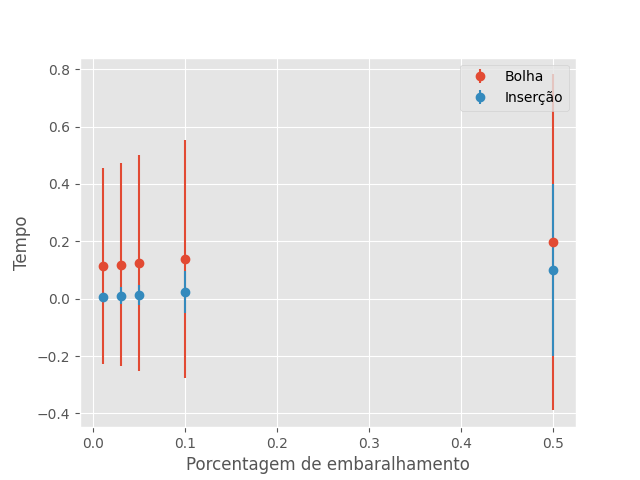
\includegraphics[width=8cm]{second}
    \caption{Gráfico elucidando o comportamento de cada algoritmo em tópico}
    \end{figure}


\section*{Conclusão}
Os algoritmos em questão, apesar de possuírem diferentes desempenhos dependendo da ordenação da lista, possuem um baixo proveito com listas muito grande. Portanto, a fim de ordenar uma lista com maior rapidez, é notável que a função built-in do Python deve, pelo menos para listas grandes, ser usada em relação aos outros métodos outrora discutidos.

\end{document}